
\chapter{Methods}

\section{EEG Preprocessing}

First, we filter the EEG signal with a notch filter at the line frequency (50Hz).
Then we apply a bandpass filter between 0.5Hz and 50Hz. 
We rereference the data.
Then we apply the ICA transform, removing artifact components and reducing the dimensionality from 128 channels to 12.
We calculate the band power for every ICA component and the standard EEG frequency bands, and concatenate the results. 
Without this step, we observe that the models struggle to train.
Before concatenation, we apply z-score normalization per frequency band.

\begin{figure}[h]
  \centering
  \makebox[\textwidth]{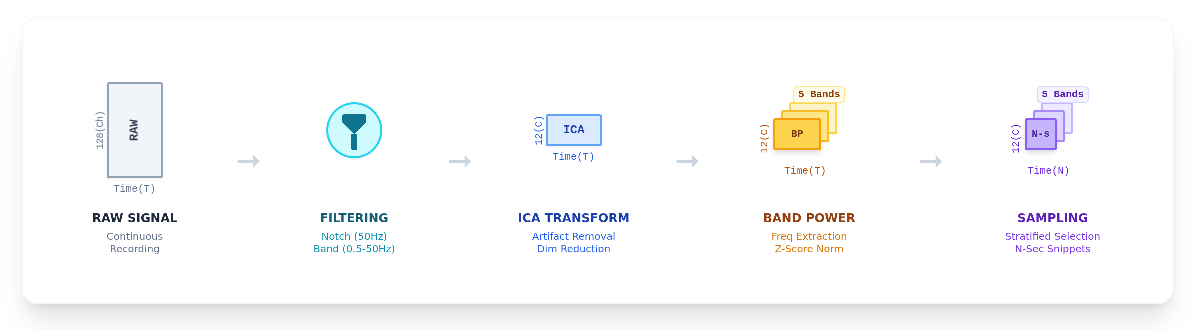
\includegraphics[width=1.1\linewidth]{imgs/preprocessing_pipeline.pdf}}
  \caption{EEG preprocessing pipeline.}
  \label{fig:preprocessing-pipeline}
\end{figure}

\begin{figure}[h]
  \centering
  \begin{minipage}{0.48\textwidth}
    \centering
    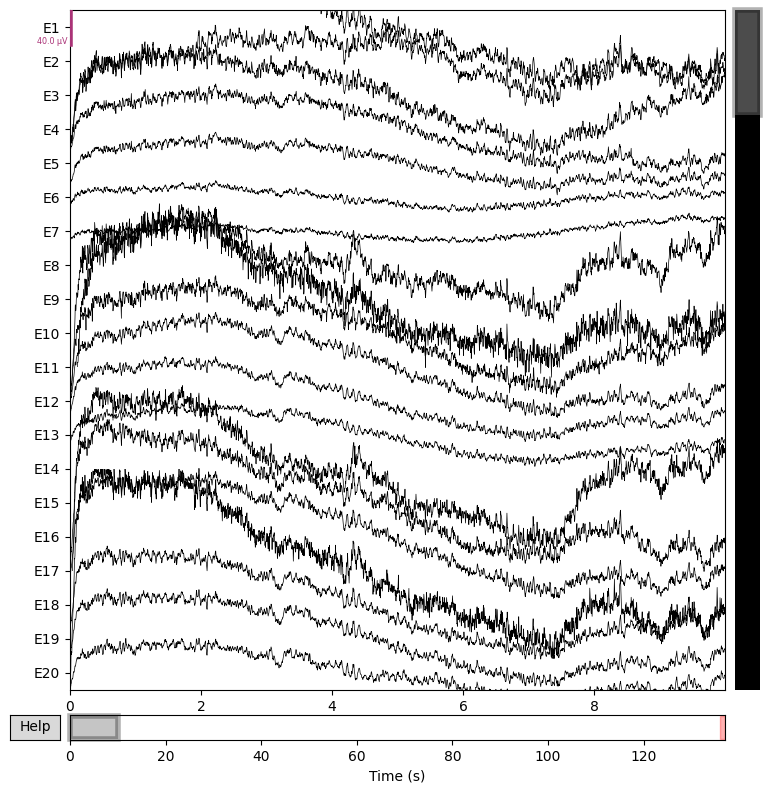
\includegraphics[width=\linewidth]{imgs/eeg_signal_10s_bl_wh.png}
    \caption{EEG signal: 10 second snippet of raw unprocessed EEG signal.}
    \label{fig:eeg-raw}
  \end{minipage}
  \hfill
  \begin{minipage}{0.48\textwidth}
    \centering
    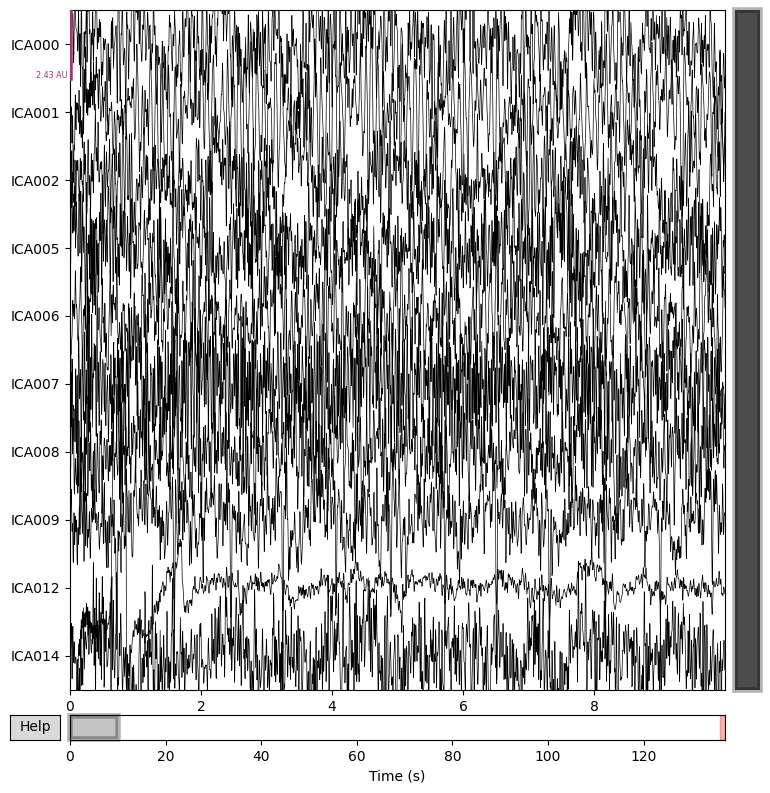
\includegraphics[width=\linewidth]{imgs/ica_signal_10s_bl_wh.png}
    \caption{EEG signal: ICA components.}
    \label{fig:eeg-ica}
  \end{minipage}
\end{figure}

\begin{figure}[h]
  \centering
  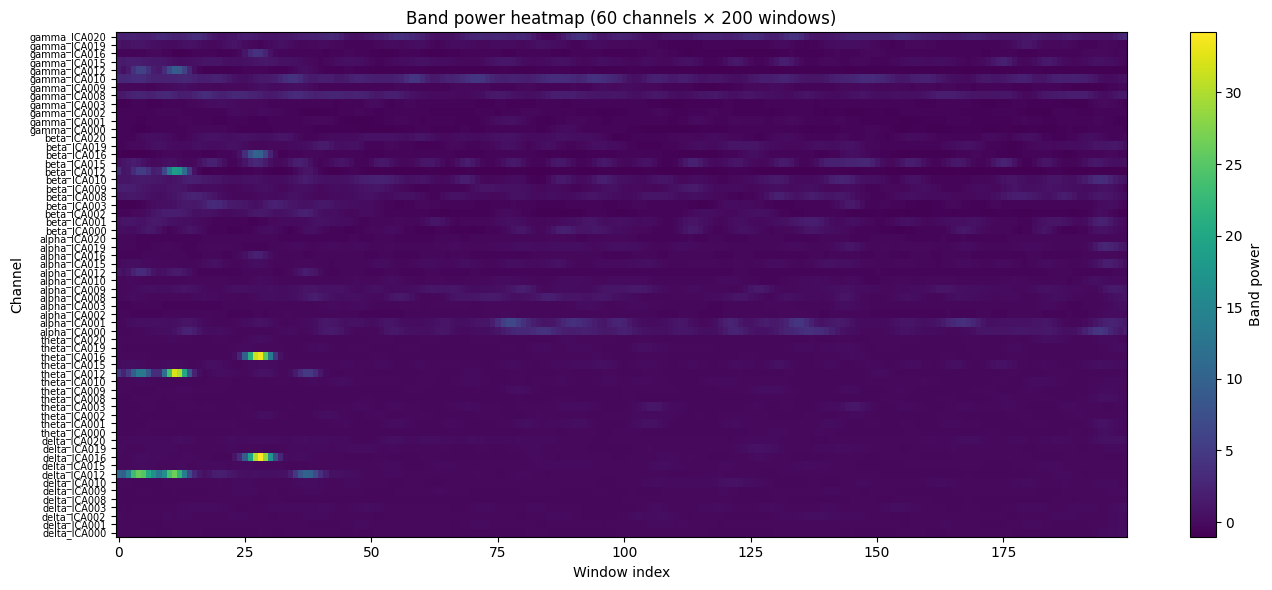
\includegraphics[width=\linewidth]{imgs/ica_band_power_20s.png}
  \caption{Band power of ICA components: 20 second snippet of preprocessed signal.}
  \label{fig:ica-band-power}
\end{figure}

During training, we sample an EEG signal snippet of 3 seconds in length from the full recording.
It was found that varying the length between 3s, 5s, 10s, and 20s impacts classification performance, with longer snippets yielding better accuracy scores\cite{pandey}.
This acts like a data augmentation method.
To avoid the Birthday Problem when randomly sampled segments often strongly overlap over part of the full recording, we 
use stratified sampling method, where first one of \( k \) segments is picked (one after another) and then a random snippet starting within chosen segment is sampled, spreading the distribution more evenly across the whole recording.

\section{Music processing}

\subsection{Spectrogram}

A music spectrogram is a visual representation of the spectrum of frequencies in a sound over time, created by applying a short-time Fourier transform (STFT) to the audio signal.
It is a 2D representation where the x-axis represents time, the y-axis represents frequency, and the intensity or color represents the magnitude of the frequency components at each point in time.
We specifically utilize mel spectrograms, which applies logarithmic scaling to the intensity values to better match human auditory perception.

\subsection{ODF function}
\label{sec:odf}

An odf function is a specific filter on a spectrogram, that responds to the intensity of change in the spectrogram over time.
So, when a spectrogram is relatively constant, the function has values close to 0 and the values are high when there's intense change in the spectrogram, 
where the higher frequency components are counted with stronger weight.

\subsection{Note onset feature extraction}
\label{sec:note-onset}

For the task of detecting note onsets, we use the essentia\cite{essentia} library with its HFC onset detection method to transform the raw wave audio signal into a list of note onset start times.
It first calculates the ODF function and then finds peaks in the function values.

\section{Models}

We use five different model types: KNN, SVM, XGBoost, a Convolutional Neural Network and an LSTM.

\subsection{KNN, SVM, XGBoost}

We employ a KNN model, where a prediction is given by an averaged values of 5 nearest neighbors in euclidean space.
SVM or Support Vector Machines model is a kernel method, where we use the 'Radial Basis Function' kernel.
The XGBoost model is a tree ensamble method, in our case 100 decision trees with a maximum depth of 6 are used together to vote for a prediction.
For a further discussion on the KNN, SVM, and XGBoost models, we refer the reader to Sarker\cite{sarker}\cite{sarker2}.

\subsection{CNN}

We define two related CNN networks: for the classification task and for the music reconstruction task.

\subsubsection{Classification CNN}

The classification network is convolutional neural network with 3 convolutional layers and a fully-connected layer.
It is designed to work with EEG images after preprocessing, which results in 1s snippets of shape \( 60\times 10\).
The model has 35,188 parameters.

% table with layers of cnn 
\begin{table}[h]
\centering
\footnotesize
\begin{tabular}{l|ll}
\hline
\textbf{Layer Type} & \textbf{Filter Size} & \textbf{Input → Output} \\
\hline
Conv2D (freq) & $1 \times 5$ & $[B, 1, 60, 10] \to [B, 16, 60, 10]$ \\
BatchNorm2D & - & $''$ \\
Conv2D (time) & $5 \times 1$ & $[B, 16, 60, 10] \to [B, 32, 60, 10]$ \\
ELU & - & $''$ \\
MaxPool2D & $2 \times 2$ & $[B, 32, 60, 10] \to [B, 32, 30, 5]$ \\
Dropout & - & $''$ \\
\hline
Conv2D (freq) & $1 \times 3$ & $[B, 32, 30, 5] \to [B, 64, 30, 5]$ \\
BatchNorm2D & - & $''$ \\
Conv2D (time) & $3 \times 1$ & $[B, 64, 30, 5] \to [B, 128, 30, 5]$ \\
ELU & - & $''$ \\
MaxPool2D & $2 \times 2$ & $[B, 128, 30, 5] \to [B, 128, 15, 2]$ \\
Dropout & - & $''$ \\
\hline
Conv2D (freq) & $1 \times 3$ & $[B, 128, 15, 2] \to [B, 128, 15, 2]$ \\
BatchNorm2D & - & $''$ \\
Conv2D (time) & $3 \times 1$ & $''$ \\
ELU & - & $''$ \\
MaxPool2D & $2 \times 2$ & $[B, 128, 15, 2] \to [B, 128, 7, 1]$ \\
Dropout & - & $''$ \\
\hline
Flatten & - & $[B, 128, 7, 1] \to [B, 896]$ \\
Linear & - & $[B, 896] \to [B, 4]$ \\
\hline
\end{tabular}
\caption{CNNClassifier model: Classifier model trained on band power data.}
\label{tab:cnn-layers}
\end{table}

\subsubsection{Reconstruction CNN}

The reconstruction network uses a U-Net style architecture with a 3-layer contracting encoder, a middle bottleneck fully connected layer, and a 3-layer expanding decoder.
The encoder has the same architecture as the classifier model, and the decoder is correspondingly a 3-layer upsampling convolutional network.
There are skip connections between matching layers of the encoder and decoder.
Because the input has a different dimensionality than the output and consequently, the outputs of the encoder and decoder layers differ in shape, the skip connections also apply interpolation to match the dimensions.
The model has 143,280 parameters.

We also define a simplified version of the reconstruction network, which aims to reconstruct spectrograms which are constant in the time dimension.
This significantly reduces complexity and allows to remove decoder part of the model.
Both full (CNNReconstruction) and simplified (CNNReconstructionMel) architectures are visible in Figure~\ref{fig:cnn-diagrams}.

\begin{figure}[h]
  \centering
  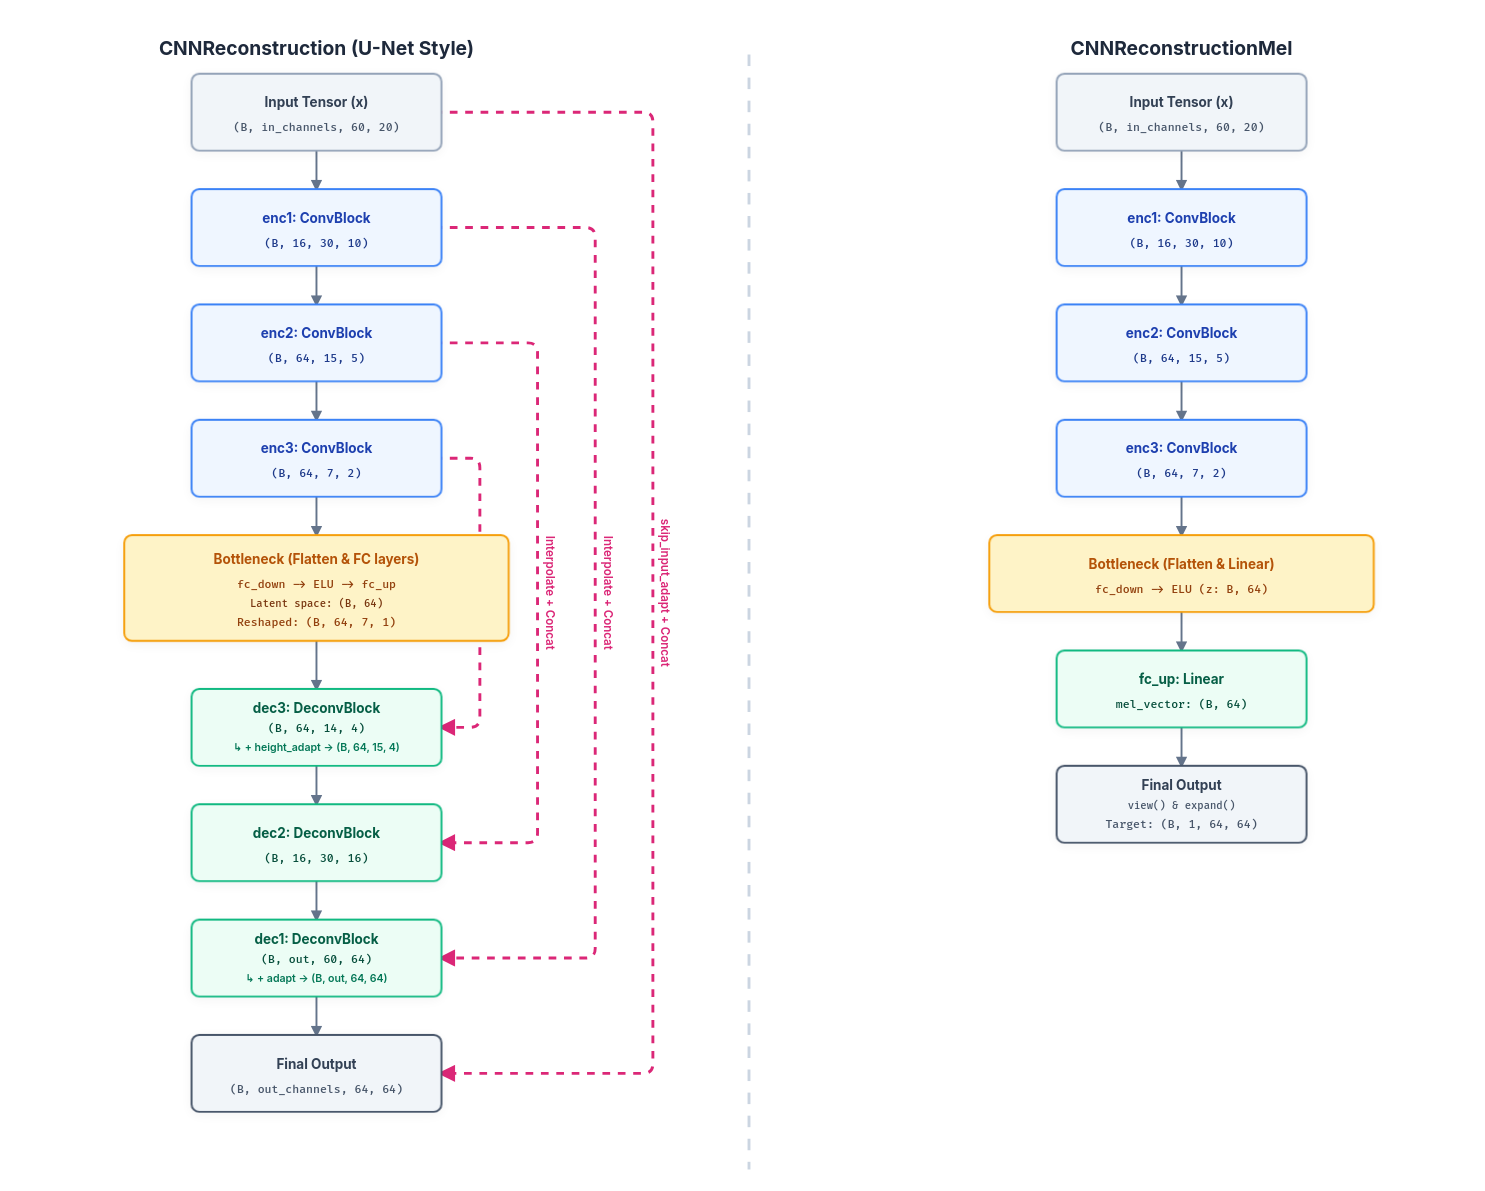
\includegraphics[width=\textwidth]{imgs/cnn_diagrams.png}
  \caption{Architecture diagrams of the full reconstruction CNN (U-Net style with encoder, bottleneck, and decoder with skip connections) and the simplified time-constant variant (encoder followed by a single fully connected layer producing a $64\times1$ output broadcasted to $64\times64$).}
  \label{fig:cnn-diagrams}
\end{figure}

\begin{table}[h]
\centering
\footnotesize
\begin{tabular}{l|ll}
\hline
\textbf{Layer Type} & \textbf{Filter Size} & \textbf{Input → Output} \\
\hline
\multicolumn{3}{c}{\textit{Encoder}} \\
\hline
Conv2D (freq) & $1 \times 5$ & $[B, 1, 60, 10] \to [B, 16, 60, 10]$ \\
BatchNorm2D & - & $''$ \\
Conv2D (time) & $5 \times 1$ & $[B, 16, 60, 10] \to [B, 32, 60, 10]$ \\
ELU & - & $''$ \\
MaxPool2D & $2 \times 2$ & $[B, 32, 60, 10] \to [B, 32, 30, 5]$ \\
Dropout & - & $''$ \\
\hline
Conv2D (freq) & $1 \times 3$ & $[B, 32, 30, 5] \to [B, 64, 30, 5]$ \\
BatchNorm2D & - & $''$ \\
Conv2D (time) & $3 \times 1$ & $[B, 64, 30, 5] \to [B, 128, 30, 5]$ \\
ELU & - & $''$ \\
MaxPool2D & $2 \times 2$ & $[B, 128, 30, 5] \to [B, 128, 15, 2]$ \\
Dropout & - & $''$ \\
\hline
Conv2D (freq) & $1 \times 3$ & $[B, 128, 15, 2] \to [B, 128, 15, 2]$ \\
BatchNorm2D & - & $''$ \\
Conv2D (time) & $3 \times 1$ & $''$ \\
ELU & - & $''$ \\
MaxPool2D & $2 \times 2$ & $[B, 128, 15, 2] \to [B, 128, 7, 1]$ \\
Dropout & - & $''$ \\
\hline
\multicolumn{3}{c}{\textit{Bottleneck}} \\
\hline
Flatten & - & $[B, 128, 7, 1] \to [B, 896]$ \\
Linear + ELU & - & $[B, 896] \to [B, 128]$ \\
Unsqueeze & - & $[B, 128] \to [B, 128, 1, 1]$ \\
ConvTranspose2D & $7 \times 1$ & $[B, 128, 1, 1] \to [B, 128, 7, 1]$ \\
\hline
\multicolumn{3}{c}{\textit{Decoder}} \\
\hline
Concat (skip enc3) & - & $[B, 128, 7, 1] + [B, 128, 7, 1] \to [B, 256, 7, 1]$ \\
Upsample & $2 \times 4$ & $[B, 256, 7, 1] \to [B, 256, 14, 4]$ \\
Conv2D (time) & $3 \times 1$ & $[B, 256, 14, 4] \to [B, 128, 14, 4]$ \\
BatchNorm2D & - & $''$ \\
Conv2D (freq) & $1 \times 3$ & $''$ \\
ELU & - & $''$ \\
Dropout & - & $''$ \\
AdaptiveAvgPool2D & - & $[B, 128, 14, 4] \to [B, 128, 15, 4]$ \\
\hline
Concat (skip enc2) & - & $[B, 128, 15, 4] + [B, 128, 15, 4] \to [B, 256, 15, 4]$ \\
Upsample & $2 \times 4$ & $[B, 256, 15, 4] \to [B, 256, 30, 16]$ \\
Conv2D (time) & $3 \times 1$ & $[B, 256, 30, 16] \to [B, 64, 30, 16]$ \\
BatchNorm2D & - & $''$ \\
Conv2D (freq) & $1 \times 3$ & $[B, 64, 30, 16] \to [B, 32, 30, 16]$ \\
ELU & - & $''$ \\
Dropout & - & $''$ \\
\hline
Concat (skip enc1) & - & $[B, 32, 30, 16] + [B, 32, 30, 16] \to [B, 64, 30, 16]$ \\
Upsample & $2 \times 4$ & $[B, 64, 30, 16] \to [B, 64, 60, 64]$ \\
Conv2D (time) & $5 \times 1$ & $[B, 64, 60, 64] \to [B, 16, 60, 64]$ \\
BatchNorm2D & - & $''$ \\
Conv2D (freq) & $1 \times 5$ & $[B, 16, 60, 64] \to [B, 1, 60, 64]$ \\
ELU & - & $''$ \\
Dropout & - & $''$ \\
\hline
\multicolumn{3}{c}{\textit{Final Adaptation}} \\
\hline
Conv2D + ELU & $3 \times 3$ & $[B, 1, 60, 64] \to [B, 1, 60, 64]$ \\
AdaptiveAvgPool2D & - & $[B, 1, 60, 64] \to [B, 1, 64, 64]$ \\
Concat (skip input) & - & $[B, 1, 64, 64] + [B, 1, 64, 64] \to [B, 2, 64, 64]$ \\
Conv2D & $1 \times 1$ & $[B, 2, 64, 64] \to [B, 1, 64, 64]$ \\
\hline
\end{tabular}
\caption{CNNReconstruction model: U-Net style network for music spectrogram reconstruction.}
\label{tab:cnn-reconstruction-layers}
\end{table}


\subsection{DTW}

DTW is an algorithm that finds an optimal alignment between two sequences.

We employ a generalized version called approximate-subsequence-DTW, which can be defined by:
\begin{enumerate}
  \item Given two sequences $A$ and $B$, it finds a match between an infix of $A$ and infix of $B$.
  \item The summed distances between the matched points are within the cost allowance.
  \item The matched infix is of maximal length.
\end{enumerate}

This means that the algorithm pairs points from one sequence, or just an infix of it, with points from the other sequence.
As many points are matched as is possible within the cost constraint, which specifies what is the sum of differences between the matched points.
The algorithm is a variant of the standard DTW dynamic programming algorithm.

\subsection{LSTM}

LSTM, or more specifically Bi-LSTM (an LSTM with bidirectional information flow), is a recurrent neural network operating on raw EEG timeseries.
We use variants operating on 12 or 129 EEG channels, with 2 hidden layers and 256 hidden units.
The output of the network is a scalar.

% \section{Neurals Networks}

% \section{XGBoost}

% \section{SVM}

% https://pubmed.ncbi.nlm.nih.gov/40039043/

% \section{KNN}
